\scanpage{115}
\mspage{2}

On introduit des sommets
\[
(6)\qquad R_r^{i,j}\qquad r\in\mathcal{R},\quad (i,j)\in\operatorname{Rep}\{0,1,\infty\}\quad\text{i.e. }i,j\in\{0,1,\infty\},\ i\ne j
\]
comme indi\uline{qués, satisfaisant} aux seules relations
\[
(7)\qquad
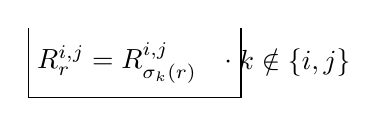
\begin{tikzpicture}[baseline=(relation.base)]
  \node[inner xsep=3pt,inner ysep=5pt] (relation)
    {$R_r^{i,j}=R_{\sigma_k(r)}^{i,j}\quad\cdot$};
  \draw[line width=.45pt] (relation.north west) -- (relation.south west)
    -- (relation.south east) -- (relation.north east);
  \node[anchor=west,inner sep=0pt,xshift=-1pt] at (relation.east)
    {$k\notin\{i,j\}$};
\end{tikzpicture}
\]
On dit que $R_r^{ij}$ est ``proche'' du
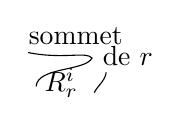
\begin{tikzpicture}[baseline=(baseR.base)]
  \node[anchor=base west,inner sep=0pt] (baseR) at (0,0) {$R_r^i$};
  \node[anchor=base west,inner sep=0pt] at (-.20,.59) {\inserted{sommet}};
  \node[anchor=base west,inner sep=0pt] at (.74,.33) {\inserted{de $r$}};
  \draw[line width=.4pt] (-.20,.49) .. controls (.25,.40) and (.54,.51) .. (.61,.42)
    .. controls (.52,.25) and (-.08,.31) .. (-.10,.06);
  \draw[line width=.4pt] (.79,.24) .. controls (.78,.13) and (.67,.06) .. (.64,-.02);
\end{tikzpicture}
($=R_s,R_o,R_f$ suivant que $i=0,1,\infty$), il se trouve sur le côté
\deleted{\unsure{du plus proche}} \inserted{qui joint celui-ci}
\deleted{\illegible{1} \unsure{repère} opposé} au sommet de type $j$.

On introduit des arcs
\[
(8)\qquad \lambda_r^i:R_r^{i,i+1,}\longrightarrow R_r^{i,i+2}\qquad r\in\mathcal{R},\ i\in\{0,1,\infty\}
\]
\[
(9)\qquad a_r^i:R_r^{i\deleted{\unsure{+2|i+2}},i+1}\longrightarrow R_r^{i+1,i+2}\qquad r\in\mathcal{R},\ i\in\{0,1,\infty\}
\]
\margin{\uline{NB} On écrit pour simplifier $i+1$ au lieu du résultat de la permutation circulaire $(0,1,\infty)\longmapsto(1,\infty,0)$, i.e. on identifie $\{0,1,\infty\}$ à $\mathbb{Z}/3\mathbb{Z}\ldots$}

\deleted{qui}
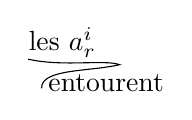
\begin{tikzpicture}[baseline=(entourent.base)]
  \node[anchor=base west,inner sep=0pt] (entourent) at (0,0) {entourent};
  \node[anchor=base west,inner sep=0pt] at (-.25,.52) {\inserted{les $a_r^i$}};
  \draw[line width=.4pt] (-.25,.41) .. controls (.19,.31) and (.73,.41) .. (.91,.34)
    .. controls (.52,.25) and (-.09,.29) .. (-.08,.04);
\end{tikzpicture}
le drapeau repère $r$ en formant un contour fermé dans le sens
\deleted{\uline{opposé}} \inserted{de} l'orientation de $r$ ---
\deleted{par contre} \inserted{\unsure{de = désignent}} les $\lambda_r^i$
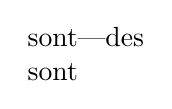
\begin{tikzpicture}[baseline=(oldverb.base)]
  \node[anchor=base west,inner sep=0pt] (oldverb) at (0,0) {\deleted{sont}};
  \node[anchor=base west,inner sep=0pt] at (0,.43) {\inserted{\unsure{sont|des}}};
\end{tikzpicture}
\deleted{\unsure{une}} portions d'arc tournant autour des sommets de $r$ de type $i$
dans le sens correspondant à l'orientation de $r$.
(Cela \deleted{\unsure{nous}} semble préférable à la convention de notation inverse).
On a les seules \deleted{identités} redondances
\[
(10)\qquad \boxed{a_r^i=a_{\tau_i(r)}^i}
\]
\margin{\begin{tabular}{@{}l@{}}
\uline{NB} On désigne\\
par les \deleted{\unsure{ces}} lettres\\
les flèches obtenues\\
après bouchage de\\
certains trous\\
si on bouche\\
$R_r^i$,
\end{tabular}}
\margin{\begin{tabular}{@{}l@{}}
(\uline{NB} si\\
les disques où\\
$\lambda_r^i$ devient $=1$)
\end{tabular}}

\deleted{On désigne}

\uline{NB} On supposera que la carte combinatoire se trouve réalisée par sa réalisation conforme canonique, qui est une surface $\unsure{\mathbb{C}|\mathcal{C}}$ analytique réelle donc $C^\infty$, dont on peut considérer son éclaté en les $R_\varphi$ $(\varphi\in S)$ et le découpe de l'éclaté, qui est une surface à bord analytique réelle (mais pas conforme) dont l'intérieur coïncide avec $X\setminus S$, on le note

\mspage{114}
